% =====================================================================
% Appendix A: TAXI datasheet and why TAXI (one-column appendix).
% All numbers are measured on the cstbench v0.1.0 build of BAS TAXI 2.5.
% Licence: no TAXI audio, transcript, translation or system output may appear.
% Floats: tab:taxi-full, fig:taxi-stats, fig:taxi-session, tab:corpora.
% =====================================================================
\section{TAXI Datasheet and Why TAXI}\label{app:taxi}

This appendix documents \taxi, the real track of \bench (\cref{sec:bench}), and explains why it is built from TAXI. \Cref{tab:taxi-full} lists its statistics, \cref{fig:taxi-stats} shows their distributions and \cref{fig:taxi-session} shows one rendered session. Because TAXI may not be redistributed, we report aggregates only: no TAXI audio, transcript or translation appears in this paper, its figures or the released files.

% =====================================================================
% Table A1 (tab:taxi-full): full TAXI datasheet statistics. Included from App. A.
% All values are measured on the cstbench v0.1.0 build of BAS TAXI 2.5.
% The last block (rendered sessions) holds the per-condition rows that the
% compact Table 2 drops; the values also appear in the App. A text.
% "--" marks cells that are not applicable or not reported (no derived sums).
% One pending row (\tbd): the silence between the energetic frames of two
% turns at speaker changes, which is 0.2 s longer than the drawn gap unless a
% margin was cut at a file edge (review: report both; computable from the
% timelines, not measured yet). Do not fill it with drawn gap + 0.2.
% =====================================================================
\begin{table}[htbp]
  \caption{Full statistics of the \taxi build (\texttt{cstbench} v0.1.0). Rendered turns are the 16\,kHz turns after silence trimming, 0.1\,s margins included; they are identical in L0 natural and L0 mediated. Untrimmed values refer to the usable source turn files. Turn files exclude pre-dialogue and hang-up items. Same-speaker successions: 9 arise because unusable turns between them were skipped, 5 are adjacent in the source. Reference words are those of the human translations of the column's turns. Marks (SpeechDat notation): * hardly recognisable, \textasciitilde{} truncated, ** unintelligible. Percentiles use linear interpolation; the scorer's p90 of $m$ values instead takes the sorted value at the 0-based index $\min(m-1,\lfloor 0.9m\rfloor)$ (\cref{app:scorer}). --: not applicable or not reported; blank: pending.}
  \label{tab:taxi-full}
  \centering
  \small
  \begin{tabular}{@{}lccc@{}}
    \toprule
    Statistic & \makecell{German\\(dispatcher)} & \makecell{English\\(client)} & All \\
    \midrule
    \multicolumn{4}{@{}l}{\textit{Sessions and turns}} \\
    Sessions                                               & --                  & --                   & 86                  \\
    Turn files                                             & 374                 & 323                  & 697                 \\
    Usable turns                                           & 349                 & 291                  & 640 (91.82\%)       \\
    Unusable turns (skipped when rendering)                & 25                  & 32                   & 57                  \\
    Sessions with $\geq 1$ unusable turn                   & --                  & --                   & 40                  \\
    Usable turns per session: median (mean; range)         & 4 (4.06; 1--9)      & 3 (3.38; 0--8)       & 7 (7.44; 1--17)     \\
    Sessions opened by this speaker (first usable turn)    & 85                  & 1                    & --                  \\
    Direction switches: total (per session: median; range) & --                  & --                   & 540 (6; 0--14)      \\
    Same-speaker successions (skipped\,/\,adjacent)        & --                  & --                   & 14 (9\,/\,5)        \\
    \midrule
    \multicolumn{4}{@{}l}{\textit{Audio}} \\
    Usable turn audio before trimming (min)                & 24.563              & 28.068               & 52.631              \\
    Speech after trimming (min)                            & 17.953              & 22.425               & 40.378              \\
    Untrimmed turn (s): mean\,/\,median\,/\,p90            & 4.223\,/\,3.64\,/\,7.02 & 5.787\,/\,4.76\,/\,10.94 & 4.934\,/\,4.0\,/\,9.064 \\
    Rendered turn (s): mean\,/\,median                     & 3.086\,/\,2.42      & 4.624\,/\,3.38       & 3.785\,/\,2.86      \\
    Rendered turn (s): p90\,/\,max                         & 5.492\,/\,12.64     & 9.92\,/\,17.98       & 7.76\,/\,17.98      \\
    Rendered turns longer than 5\,s                        & --                  & --                   & 144 (22.5\%)        \\
    Rendered turns longer than 10\,s                       & --                  & --                   & 29 (4.5\%)          \\
    Silence removed per turn (s): median leading\,/\,trailing & 0.5\,/\,0.46     & 0.56\,/\,0.44        & 0.54\,/\,0.44       \\
    Speaking rate (words/s): trimmed (untrimmed) audio     & 2.997 (2.19)        & 2.666 (2.13)         & --                  \\
    \midrule
    \multicolumn{4}{@{}l}{\textit{Text}} \\
    Source words                                           & 3,228               & 3,587                & 6,815               \\
    Source words per turn: mean\,/\,median\,/\,p90\,/\,max & 9.25\,/\,8\,/\,17\,/\,34 & 12.33\,/\,10\,/\,25\,/\,37 & --         \\
    Reference words                                        & 3,339               & 3,278                & 6,617               \\
    Reference words per turn: mean\,/\,median\,/\,max      & 9.57\,/\,8\,/\,44   & 11.26\,/\,10\,/\,38  & --                  \\
    Vocabulary, source\,/\,reference (lowercased types)    & 472\,/\,381         & 534\,/\,602          & --                  \\
    Filled-pause marks [fil]                               & 60                  & 172                  & --                  \\
    Noise labels (NOI tier)                                & 235                 & 228                  & --                  \\
    Other marks: *\,/\,\textasciitilde\,/\,**              & 53\,/\,8\,/\,1      & 61\,/\,4\,/\,11      & --                  \\
    Turns containing markup                                & 101                 & 135                  & --                  \\
    \midrule
    \multicolumn{4}{@{}l}{\textit{Rendered sessions, L0 natural\,/\,L0 mediated (gaps as drawn, between margin-inclusive turns)}} \\
    Session audio (h)                                      & --                  & --                   & 0.737\,/\,0.998     \\
    Median session (s)                                     & --                  & --                   & 29.023\,/\,39.316   \\
    Speaker-change gap (s): mean\,/\,median, natural       & --                  & --                   & 0.257\,/\,0.223     \\
    Speaker-change gap (s): mean\,/\,median, mediated      & --                  & --                   & 1.995\,/\,2.026     \\
    Natural gaps at the 0.05\,s floor                      & --                  & --                   & 129 (23.89\%)       \\
    Speaker-change silence between speech (s): median      & --                  & --                   & \tbd                \\
    Speech occupancy (\%)                                  & --                  & --                   & 91.27\,/\,67.42     \\
    Overlap ratio                                          & --                  & --                   & 0.0\,/\,0.0         \\
    \bottomrule
  \end{tabular}
\end{table}


\paragraph{Source and usable turns.}
BAS TAXI~2.5 \citep{bas2001taxi}, distributed through the BAS CLARIN repository \citep{reichel2016bas}, holds telephone dialogues between a German-speaking taxi dispatcher and an English-speaking client, each speaking their own language. Every turn is a separate 8\,kHz, 16-bit mono file. Speakers took turns with a push-to-talk button, which prevented overlap and kept no inter-turn timing, so only the order of the turns is known. Turns that passed the corpus validation carry a BAS Partitur annotation with orthographic words in SpeechDat notation (ORT tier), pronunciations (KAN), noise labels (NOI) and a human translation into the other language (TLN); turns rated as garbage (overlapping speech, meta talk, empty, noise only or wrong language) have none. We drop pre-dialogue and hang-up items, which leaves 697 dispatcher and client turn files in 86 sessions (IDs SES0037--SES0130, not contiguous), and keep a turn if its cleaned transcript is non-empty and it has a human translation whose direction matches the speaker's language. Cleaning removes bracketed markers such as [fil] and unintelligible tokens (**), strips the marks of hardly recognisable (*) and truncated (\textasciitilde) words, and keeps word fragments. This leaves 640 usable turns (91.82\%; German 349, English 291), exactly the turns that the validation list shipped with the corpus marks usable; 40 sessions contain at least one unusable turn, which the renderer skips. The corpus README reports 645 usable turns from the original validation, and the corpus's revalidation report counts 640, as we do; catalogue entries give 94 dialogues, the number recorded, but version~2.3 removed the eight that have no usable turn. The build identifies speakers only by role, so we report no speaker counts or demographics.
\draftnote{add speaker counts, recording conditions and translation guidelines from the corpus documentation}

\paragraph{Composition.}
German turns are shorter than English ones: after silence trimming, the median turn lasts 2.42\,s in German and 3.38\,s in English, and the median number of source words per turn is 8 and 10. The rendered turns amount to 40.378\,min of speech after silence trimming (52.631\,min of usable turn audio before trimming). Over both languages, the median turn lasts 2.86\,s, 22.5\% of the turns exceed 5\,s and 4.5\% exceed 10\,s (\cref{fig:turn-length} breaks latency down by turn length). On trimmed audio, the speaking rate is 2.997 words/s in German and 2.666 words/s in English. The transcripts mark what synthetic speech lacks: 60 German and 172 English filled pauses and 8 and 4 truncated words, and the NOI tier holds 235 and 228 noise labels. The human translations are lowercase and unpunctuated, so the scorer normalises hypotheses to this style (\cref{app:scorer}). Each direction has only about 3.3k reference words (3,339 English words for the German turns and 3,278 German words for the English turns), so every comparison uses session-clustered bootstrap intervals (\cref{app:repro}).

\paragraph{Rendering.}
The build resamples the usable turns from 8 to 16\,kHz with a polyphase filter and keeps the telephone band; it applies no bandwidth extension, which matters when reading ASR error rates. It trims each turn to the span from the first to the last 20\,ms frame whose RMS exceeds a threshold of 0.1 times the 95th-percentile frame RMS (but at least $10^{-4}$), widened by a 0.1\,s margin on each side. Trimming removes a median of 0.54\,s of leading and 0.44\,s of trailing silence per turn; the totals, 416.06\,s and 319.14\,s, account exactly for the difference between the untrimmed (3157.86\,s) and the trimmed audio (2422.66\,s).\draftnote{a median leading silence of 0.88\,s (about 0.9\,s in the code docstring) is not reproduced by this build; do not quote it}
Only the timing is sampled, as in simulated conversations for diarization training \citep{landini2022from}; the turns and their order are real. The renderer places the turns in dialogue order after a 0.5\,s lead, separates consecutive turns of one speaker by a pause drawn from $\mathcal{U}[0.3,0.8]$\,s, appends a 0.5\,s tail and sums the two speaker channels, clipped to $[-1,1]$. At a speaker change, L0 natural draws the gap from $\mathcal{N}(0.2,0.25^2)$\,s clipped to $[0.05,1.0]$\,s, close to the typical gap of about 200\,ms \citep{levinson2015timing}, which varies little across languages \citep{stivers2009universals}; L0 mediated draws it from $\mathcal{U}[1,3]$\,s, for a listener who reads the translation before answering. At the 540 speaker changes, natural gaps have a mean of 0.257\,s and a median of 0.223\,s, and 129 of them (23.89\%) sit at the 0.05\,s floor, against about 27.4\% expected from clipping the normal; mediated gaps have a mean of 1.995\,s and a median of 2.026\,s (\cref{fig:taxi-stats}c). The renders last 0.737\,h (natural; median session 29.023\,s; speech occupancy 91.27\%) and 0.998\,h (mediated; 39.316\,s; 67.42\%), and the overlap ratio is 0.0 in all 86 sessions of both. Real conversation overlaps at many speaker changes \citep{heldner2010pauses}; L1 therefore starts the next turn $\mathcal{U}[0.2,0.8]$\,s before the previous one ends at each speaker change, under its own configuration name and checksums.
\draftnote{planned; the L1 renderer is not built yet}

\begin{figure}[htbp]
  \centering
  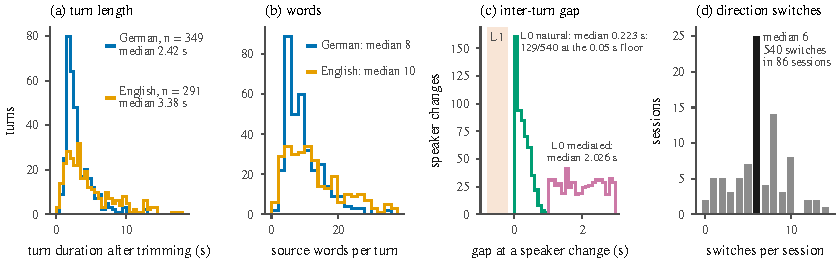
\includegraphics{figures/figA1_taxi_stats.pdf}
  \caption{\taxi statistics (86 sessions, 640 usable turns; aggregates only, as TAXI may not be redistributed). (a)~Turn duration after silence trimming (0.1\,s margins included), by source language. (b)~Source words per turn. (c)~Gaps drawn at the 540 speaker changes under L0 natural and L0 mediated; the shaded band of negative gaps marks where the planned L1 condition starts the next turn, 0.2--0.8\,s before the previous turn ends. (d)~Direction switches per session; the median (6) is drawn in black, and two sessions have no switch.}
  \label{fig:taxi-stats}
\end{figure}

\begin{figure}[htbp]
  \centering
  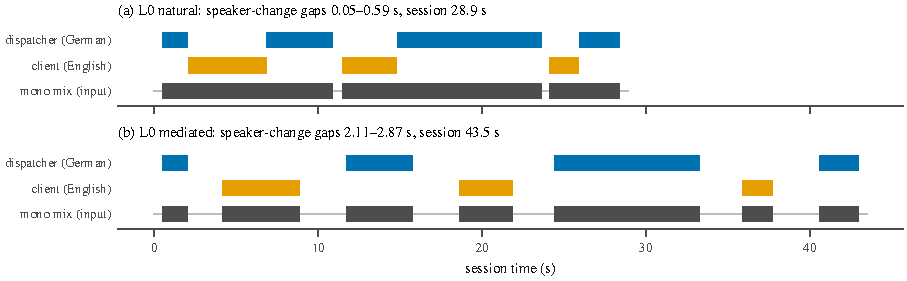
\includegraphics{figures/figA2_taxi_session.pdf}
  \caption{Session SES0104 (7 turns) rendered under (a)~L0 natural (speaker-change gaps 0.05--0.59\,s; session 28.9\,s, close to the median session of 29.023\,s) and (b)~L0 mediated (gaps 2.11--2.87\,s; session 43.5\,s). Lanes show the German dispatcher, the English client and the mono mix, which is all a system receives. Speech and turn order are real; the timing is synthetic. Only turn intervals are shown, no audio or text.}
  \label{fig:taxi-session}
\end{figure}

\paragraph{Caveats.}
Speech, content and turn order are real, but every gap is synthetic and the corpus has no overlap; overlap claims therefore rest on the L1 renders and on \syn (\cref{app:syn}). Turn intervals include the 0.1\,s margins, so the turn boundaries to which \eo and switch latency refer can be off by up to about 0.1\,s, and energy trimming may clip soft onsets; forced-aligned word times will check these boundaries.\draftnote{planned; the TAXI turns are not force-aligned yet}
Language and role are confounded (German is always the dispatcher), and the dispatcher opens 85 of the 86 sessions, a trivial prior for the first direction. The realistic wrappers therefore route by spoken-language identification (\cref{app:baselines}), and \syn renders both speaker--language assignments. Sessions SES0085 and SES0095 hold a single usable turn, in German; they have no direction switch and are excluded from switch metrics. Fourteen turns follow a turn of the same speaker, 9 because unusable turns in between were skipped and 5 because the two turns are adjacent in the source; a pause separates them, and they do not count as switches. Finally, TAXI serves only for evaluation: no threshold, operating point or model is tuned on it.

\paragraph{Release and reproducibility.}
TAXI is free of charge under a scientific licence, and a commercial licence is available; redistribution, even in part, requires the written permission of the copyright holders. We therefore release session and turn IDs, configurations, build scripts, checksums and per-turn scores keyed by turn ID, but no audio, text or system output derived from TAXI (\cref{tab:licences}). Each rendered session directory holds \texttt{mix.wav} (the single-channel system input), \texttt{2ch.wav} (one channel per speaker, for analysis and oracle diagnostics only) and \texttt{timeline.json} (turn intervals with margins, gaps, removed silence, transcripts and references). The channel order of \texttt{2ch.wav} follows the \texttt{channels} field of the timeline: channel~0 is the English client and channel~1 the German dispatcher.\draftnote{the package README states the reverse order; fix it before release}
Per-session seeds derived from the session IDs and Python's \texttt{random} module make the timelines identical on every platform (\cref{sec:bench}). \texttt{cstbench verify} requires the SHA-256 digest of every timeline (as sorted-key JSON) to match exactly and reports audio-hash differences separately, because audio hashes can depend on the numpy, scipy and libsndfile versions (the reference hashes were made with numpy 1.24.3, scipy 1.10.1 and libsndfile 1.2.2). A local rebuild matched 86/86 timeline digests and 86/86 \texttt{mix.wav} and \texttt{2ch.wav} hashes in both configurations. Released configurations are frozen, and any change gets a new name. With the corpus in \texttt{TAXI\_DIR} (one folder per session), the track is built and verified by
{\small
\begin{verbatim}
cstbench build-taxi --root TAXI_DIR --out OUT_DIR
cstbench verify --out OUT_DIR/taxi-natural  --reference checksums/taxi-natural.json
cstbench verify --out OUT_DIR/taxi-mediated --reference checksums/taxi-mediated.json
\end{verbatim}
}

\paragraph{Why TAXI.}
A real \task test set needs one conversation between at least two real speakers who use different languages, with shared multi-turn context, per-turn audio, the identity and language of each speaker, turn order and transcripts; reference translations, turn timing, session audio and per-speaker channels are desirable. Parallel speech read from scripts, separately recorded sides of a text dialogue, merged monolingual corpora and utterance sets whose order or context cannot be recovered do not qualify. \Cref{tab:corpora} checks the candidates against these requirements. MSLT \citep{federmann2016microsoft,federmann2017microsoft} was recorded from bilingual calls, but the English side of each call was discarded. DRAL \citep{ward2023dialogs,ward2024dialogs,avila2023towards} and mDRAL \citep{seamless2023seamless} pair fragments of one-language conversations with re-enactments in the other language. InCroMin \citep{cechovic2025corpus} records real meetings between people without a common language, but they talk through machine speech translation, each participant is recorded on a separate track, and no English--German pair is included. CS-Dialogue \citep{zhou2025csdialogue} holds about 104\,h of Mandarin--English code-switching without translations. The Verbmobil~II interpreter volumes, from the Verbmobil project \citep{wahlster2000verbmobil}, contain German--English and German--Japanese dialogues and a human-interpreter subset but require a paid licence, and the Fisher--CALLHOME Spanish--English corpus \citep{post2013improved} has a single source language. Among these candidates, only TAXI combines real two-language dialogues, human translations of both sides and free access for research. What it lacks, turn timing and overlap, is exactly what the renderer controls.

% =====================================================================
% Table A13 (tab:corpora): why TAXI. Real bilingual conversational speech
% resources checked against the requirements of a real CST test set.
% Included from App. A; the citation of every row is given in the text of App. A.
% Uses >{...}p{} columns (array package, loaded by makecell).
% =====================================================================
\begin{table}[htbp]
  \caption{Why \taxi: real bilingual conversational speech resources checked against the requirements of a real \task test set (citations in the text of \cref{app:taxi}). \cmark{} yes, \pmark{} partly, \xmark{} no; --: not assessed or not applicable.}
  \label{tab:corpora}
  \centering
  \footnotesize
  \setlength{\tabcolsep}{3pt}
  \begin{tabular}{@{}>{\raggedright\arraybackslash}p{2.2cm}>{\raggedright\arraybackslash}p{2.6cm}>{\raggedright\arraybackslash}p{1.4cm}>{\raggedright\arraybackslash}p{1.8cm}>{\raggedright\arraybackslash}p{2.0cm}>{\raggedright\arraybackslash}p{1.1cm}>{\raggedright\arraybackslash}p{2.0cm}>{\raggedright\arraybackslash}p{2.2cm}@{}}
    \toprule
    Corpus & Same conversation, two languages & Real spontaneous speech & Human translations & Per-turn audio\,/\,timing & Overlap & Access\,/\,licence & Verdict \\
    \midrule
    BAS TAXI 2.5
      & \cmark{} German dispatcher, English client
      & \cmark
      & \cmark{} both sides (TLN tier)
      & \pmark{} per-turn files; no timing (push-to-talk)
      & \xmark{} none
      & free scientific licence; no redistribution
      & \textbf{used} (real track) \\
    \addlinespace
    MSLT
      & \pmark{} bilingual calls; English side discarded
      & \cmark
      & \pmark{} released side only
      & one side only
      & --
      & --
      & unsuitable (one-sided release) \\
    \addlinespace
    DRAL\,/\,mDRAL
      & \xmark{} one language per conversation; fragments re-enacted in the other
      & \pmark{} originals only
      & \pmark{} spoken re-enactments
      & paired fragments
      & --
      & LDC (DRAL)
      & unsuitable (re-enacted) \\
    \addlinespace
    InCroMin
      & \cmark{} meetings mediated by machine speech translation
      & \cmark
      & \pmark{} corrected machine translations into English
      & per-participant tracks
      & --
      & CC BY 4.0
      & related work (12 languages, no English--German pair) \\
    \addlinespace
    CS-Dialogue
      & \pmark{} Mandarin--English code-switching within speakers
      & \cmark
      & \xmark
      & full dialogues
      & --
      & --
      & unsuitable (about 104\,h, no translations) \\
    \addlinespace
    Verbmobil~II interpreter volumes
      & \cmark{} German--English and German--Japanese; human-interpreter subset
      & \cmark
      & --
      & --
      & --
      & speech on paid media
      & not used \\
    \addlinespace
    Fisher--CALLHOME Spanish--English ST
      & \xmark{} one source language (Spanish)
      & \cmark
      & \cmark{} crowdsourced, into English
      & --
      & --
      & LDC
      & related (one source language) \\
    \bottomrule
  \end{tabular}
\end{table}

